\documentclass[a4paper,12pt,obeyspaces,spaces,hyphens]{article}

\usepackage{agenda}

\hypersetup{pdftitle={Formation développement noyau et pilotes Linux},
  pdfauthor={Bootlin}}

\renewcommand{\arraystretch}{2.0}

\begin{document}

\setlength{\arrayrulewidth}{0.8pt}

\begin{center}
\LARGE
Formation développement noyau et pilotes Linux\\
\large
Session de 5 jours
\end{center}
\vspace{1cm}

\small
\newcolumntype{g}{>{\columncolor{fedarkblue}}m{4cm}}
\newcolumntype{h}{>{\columncolor{felightblue}}X}

\arrayrulecolor{lightgray} {
  \setlist[1]{itemsep=-5pt}
  \begin{tabularx}{\textwidth}{|g|h|}
    {\bf Titre} & {\bf Formation développement noyau et pilotes Linux} \\
    \hline

    {\bf Aperçu} &
    Comprendre le noyau Linux \par
    Développer des pilotes de périphérique pour le noyau Linux \par
    Débogage du noyau Linux \par
    Portage du noyau Linux sur un nouveau matériel \par
    Travailler avec la communauté de développeurs du noyau Linux \par
    Travaux pratiques sur carte électronique ARM BeagleBone Black (ou
    sa variante "Wireless"). \\
    \hline
    {\bf Supports} &
    Vérifiez que le contenu de la formation correspond à vos besoins :
    \newline \url{https://bootlin.com/doc/training/linux-kernel}. \\
    \hline

    {\bf Durée} & {\bf Cinq} jours - 40 h (8 h par jour)
    \newline 50\% de présentations et 50\% de travaux pratiques. \\
    \hline

    {\bf Formateur} & Un des ingénieurs mentionnés sur :
    \newline \url{https://bootlin.com/training/trainers/}\\
    \hline

    {\bf Langue} & Présentations : Français
    \newline Supports : Anglais\\
    \hline

    {\bf Public ciblé} & Ingénieurs développant des systèmes reposant sur le noyau Linux.
    \newline Ingénieurs supportant des développeurs Linux embarqué.\\
    \hline

    {\bf Pré-requis} &

    {\bf Expérience solide en programmation en langage C}
    \newline En particulier, les participants devront maîtriser
    la création et la gestion de types et de structures de données
    complexes, de pointeurs vers de tels symboles, et de pointeurs de
    fonctions. \vspace{1em}
    \newline {\bf Connaissance et pratique des commandes UNIX ou
    GNU/Linux}
    \newline Les personnes n'ayant pas ces connaissances doivent
    s'autoformer, par exemple en utilisant nos supports de formation
    disponibles en ligne :
    \newline (\url{https://bootlin.com/blog/command-line/} \vspace{1em}
    \newline {\bf Expérience en développement Linux embarqué}.
    \newline Suivre au préalable notre Formation Linux Embarqué
    \newline (\url{https://bootlin.com/fr/formation/linux-embarque/})
    \newline n'est pas un pré-requis absolu, mais sera très utile à toutes
    personnes manquant d'expérience en Linux embarqué.
    Cela leur permettra de mieux comprendre l'environnement de
    développement et les manipulations mises en oeuvre dans les
    travaux pratiques, pour pouvoir se concentrer sur la programmation
    du code du noyau Linux.
    \\
    \hline
  \end{tabularx}

  \begin{tabularx}{\textwidth}{|g|h|}
    {\bf Équipement\newline nécessaire} &
    {\bf Pour les sessions sur site uniquement}
    \newline Le matériel est fourni par Bootlin durant les
    sessions inter-entreprises
    \begin{itemize}
    \item Projecteur vidéo
    \item Un ordinateur sur chaque bureau (pour une ou deux personnes), avec au
    moins 8 Go de RAM et Ubuntu Linux installé dans une {\bf partition
    dédiée d'au moins 20 Go. L'utilisation de Linux dans une machine virtuelle
    n'est pas supportée}, en raison de problèmes avec la connexion au matériel.
    \item Nous avons besoin d'Ubuntu Desktop 20.04 (Xubuntu et autres
    variantes fonctionnent également). Nous ne supportons pas d'autres
    distributions, car nous ne pouvons tester toutes les versions des
    paquets.
    \item {\bf Connexion à Internet} (directe ou par le proxy de l'entreprise).
    \item {\bf Les ordinateurs contenant des données importantes doivent être
    sauvegardés} avant d'être utilisés dans nos sessions. Certains
    participants ont déjà commis des erreurs lors de travaux pratiques
    avec pour conséquence des pertes de données.
    \end{itemize} \\
    \hline

    {\bf Supports} & Version électronique des présentations et travaux pratiques.
    \newline Version électronique des données pour les travaux
    pratiques..\\
    \hline

\end{tabularx}}
\normalsize

\feagendatwocolumn
{Matériel}
{
  La plateforme matérielle utilisée pendant les travaux pratiques de
  cette formation est la carte {\bf BeagleBone Black}, dont voici les
  caractéristiques :

  \begin{itemize}
  \item Un processeur ARM AM335x de Texas Instruments (à base de
    Cortex-A8), avec accélération 3D, etc.
  \item 512 Mo de RAM
  \item 2 Go de stockage eMMC embarqué sur la carte
	\newline(4 Go avec la révision C)
  \item USB hôte et device
  \item Sortie HDMI
  \item Connecteurs à 2 x 46 broches, pour accéder aux UARTs, aux
        bus SPI, aux bus I2C, et à d'autres entrées/sorties du
        processeur.
  \end{itemize}
}
{}
{
  \begin{center}
    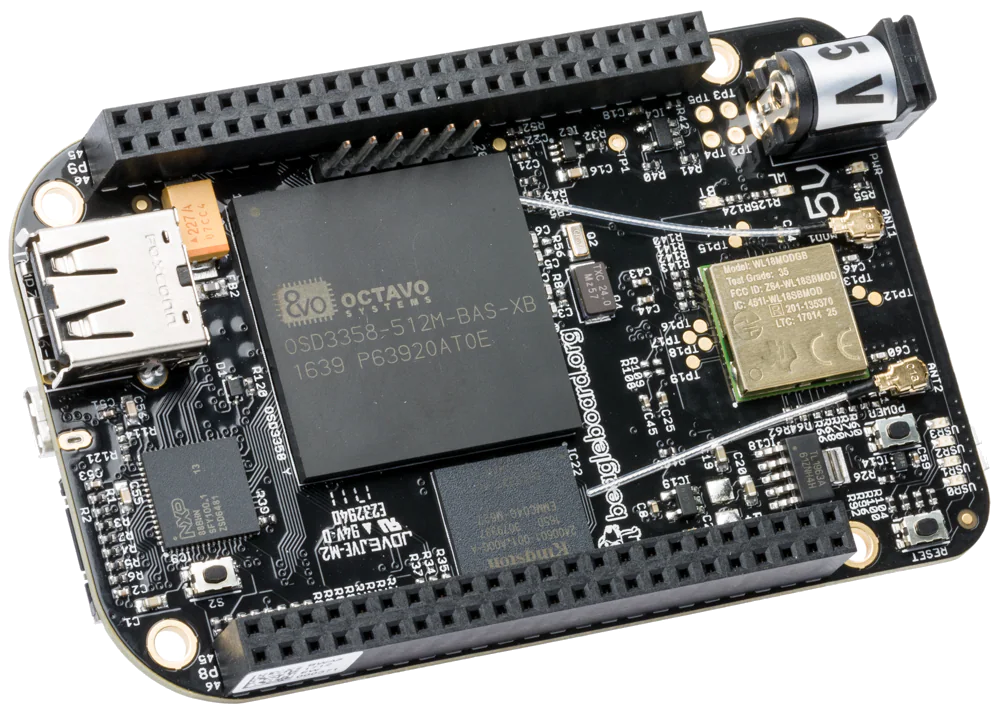
\includegraphics[height=5cm]{../slides/beagleboneblack-board/beagleboneblack.png}
  \end{center}
}

\feagendaonecolumn
{Travaux pratiques}
{
  Les travaux pratiques de cette formation font appel aux périphériques
  matériels suivants, pour illustrer le développement de pilotes de
  périphériques pour Linux :

  \begin{itemize}
  \item Une manette Nunchuk pour console Wii, qui est connectée à la
    BeagleBone Black via le bus I2C. Son pilote utilisera le
    sous-système {\em input} du noyau Linux.
  \item Un port série (UART) supplémentaire, dont les registres sont
    mappés en mémoire, et pour lequel on utilisera le sous-système {\em
    misc} de Linux.
  \end{itemize}

  Bien que nos explications cibleront spécifiquement les sous-systèmes
  de Linux utilisés pour réaliser ces pilotes, celles-ci seront toujours
  suffisamment génériques pour faire comprendre la philosophie
  d'ensemble de la conception du noyau Linux. Un tel apprentissage
  sera donc applicable bien au delà des périphériques I2C, d'entrée ou
  mappés en mémoire.
}


\section{1\textsuperscript{er} jour - Matin}

\feagendaonecolumn
{Cours - Introduction au noyau Linux}
{
  \begin{itemize}
  \item Fonctionnalités et rôle du noyau.
  \item Contraintes juridiques liées aux pilotes de périphériques.
  \item L'interface noyau / espace utilisateur (/proc et /sys).
  \item Pilotes de périphériques en espace utilisateur.
  \end{itemize}
}
\\
\feagendatwocolumn
{Cours - Les sources du noyau}
{
  \begin{itemize}
  \item Spécificités du développement noyau
  \item Conventions de codage
  \item Récupération des sources du noyau
  \item Aperçu des sources du noyau
  \item Outils de navigation dans les sources : cscope, Elixir
  \end{itemize}
}
{TP - Code source du noyau}
{
  \begin{itemize}
  \item Récupération des sources du noyau
  \item Effectuer des recherches dans les sources du noyau Linux :
    recherche de définitions C, de paramètres de configuration et d'autres
    informations.
  \item En utilisant la ligne de commande UNIX et des outils de
    navigation dans le code.
 \end{itemize}
}

\section{1\textsuperscript{er} jour - Après-midi}
\feagendatwocolumn
{Cours – Configuration, compilation et démarrage du noyau Linux}
{
  \begin{itemize}
  \item Configuration du noyau.
  \item Compilation native et croisée. Fichiers générés.
  \item Démarrage du noyau. Paramètres de démarrage.
  \item Montage du système de fichiers racine par NFS.
  \end{itemize}
}
{TP – Configuration, compilation croisée et démarrage sur NFS}
{
  {\em En utilisant la carte BeagleBone Black}
  \begin{itemize}
  \item Configuration, compilation croisée et démarrage du noyau Linux
    avec support de NFS.
  \end{itemize}
}
\\
\section{2\textsuperscript{ème} jour - Matin}

\feagendatwocolumn
{Cours – Modules noyau Linux}
{
  \begin{itemize}
  \item Pilotes de périphériques Linux
  \item Un module simple
  \item Contraintes de programmation
  \item Chargement et déchargement de modules
  \item Dépendances entre modules
  \item Ajouter du code source à l'arbre du noyau
  \end{itemize}
}
{TP - Développement de module}
{
  {\em En utilisant la carte BeagleBone Black}
  \begin{itemize}
  \item Écriture d'un module noyau offrant quelques fonctionnalités
  \item Accès aux informations internes du noyau depuis le module
  \item Mise en place de l'environnement de compilation
  \end{itemize}
}

\section{2\textsuperscript{ème} jour - Après-midi}

\feagendatwocolumn
{Lecture - Le "device model" de Linux}
{
  \begin{itemize}
  \item Comprendre comment le noyau est conçu pour supporter les pilotes
    de périphériques
  \item Le "device model"
  \item Connexion entre périphériques et pilotes.
  \item Périphériques "platform", le "Device Tree"
  \item Interface en espace utilisateur avec \code{/sys}
  \end{itemize}
}
{TP - Device model de Linux pour un pilote I2C}
{
  {\em En utilisant la carte BeagleBone Black}
  \begin{itemize}
  \item Réalisation d'un pilote qui s'enregistre comme
     un pilote I2C.
  \item Modification du Device Tree pour déclarer un
     périphérique I2C.
  \item Faire en sorte que le pilote soit appelé quand le
     périphérique I2C est énuméré au démarrage.
  \end{itemize}
}

\section{3\textsuperscript{ème} jour - Matin}

\feagendatwocolumn
{Cours - Introduction à l'API I2C}
{
  \begin{itemize}
  \item Le sous-système I2C du noyau
  \item Détails sur l'API fournie aux pilotes du noyau pour interagir
    avec les périphériques I2C.
  \end{itemize}
}
{Cours - "Pin muxing" (multiplexage d'entrées-sorties)}
{
  \begin{itemize}
  \item Comprendre l'infrastructure {\em pinctrl} du noyau.
  \item Comprendre comment configurer le multiplexage des
    entrées/sorties.
  \end{itemize}
}

\feagendaonecolumn
{TP - Communiquer avec le Nunchuk via I2C}
{
  {\em En utilisant la carte BeagleBone Black}
  \begin{itemize}
  \item Configurer le pin muxing pour le bus I2C utilisé pour
    communiquer avec le Nunchuk
  \item Étendre le pilote I2C commencé au TP précédent pour
    communiquer avec le Nunchuk à travers le bus I2C.
  \end{itemize}
}

\section{3\textsuperscript{ème} jour - Après-midi}

\feagendaonecolumn
{Cours - Infrastructures du noyau}
{
  \begin{itemize}
  \item Périphériques de type bloc et caractère
  \item Interaction entre applications en espace utilisateur et le noyau
  \item Détails sur les pilotes caractère,  \code{file_operations},
    \code{ioctl()}, etc.
  \item Échange de données vers ou depuis l'espace utilisateur
  \item Le principe des infrastructures du noyau
  \end{itemize}
}

\feagendatwocolumn
{Cours - Le sous-système input}
{
  \begin{itemize}
  \item Principe du sous-système {\em input} du noyau
  \item API offerte aux pilotes du noyau pour exposer
    des fonctionnalités de périphériques d'entrée aux
    applications en espace utilisateur.
  \item API en espace utilisateur offerte par le
    sous-système {\em input}
  \end{itemize}
}
{TP - Exposer la fonctionnalité du Nunchuk en espace utilisateur}
{
  {\em En utilisant la carte BeagleBone Black}
  \begin{itemize}
  \item Extension du pilote du Nunchuk pour exposer les fonctionnalités
    du Nunchuk aux applications en espace utilisateur, comme
    un périphérique d'entrée.
  \item S'assurer du bon fonctionnement du Nunchuk via \code{evtest}
  \end{itemize}
}

\section{4\textsuperscript{ème} jour - Matin}

\feagendatwocolumn
{Cours - Gestion de la mémoire}
{
  \begin{itemize}
  \item Linux : gestion de la mémoire. Espaces d'adressages physique et
     virtuel, séparation noyau et espace utilisateur.
  \item Implémentation de la gestion de la mémoire dans Linux.
  \item Allocation avec \code{kmalloc()}.
  \item Allocation par pages.
  \item Allocation avec \code{vmalloc()}.
  \end{itemize}
}
{Cours - Entrées-sorties avec le matériel}
{
  \begin{itemize}
  \item Enregistrement des plages de mémoire d'E/S.
  \item Accès aux plages de mémoire d'E/S.
  \item Barrières mémoire.
  \end{itemize}
}

\feagendaonecolumn
{TP - Pilote "platform" minimal et accès à la mémoire d'E/S}
{
  {\em En utilisant la carte BeagleBone Black}
  \begin{itemize}
  \item Réalisation d'un pilote "platform" minimal
  \item Modification du Device Tree pour ajouter un nouveau
    port série.
  \item Réservation des adresses d'E/S utilisées par le port série.
  \item Lecture et écriture des registres du périphérique, pour
    envoyer des caractères sur le port série.
  \end{itemize}
}

\section{4\textsuperscript{ème} jour - Après-midi}

\feagendatwocolumn
{Cours - Le sous-système misc}
{
  \begin{itemize}
  \item Utilité du sous-système {\em misc} du noyau
  \item API du sous-système {\em misc}, à la fois du côté du noyau, et
    du côté de l'espace utilisateur.
  \end{itemize}
}
{TP - Pilote de port série en écriture seule}
{
  {\em En utilisant la carte BeagleBone Black}
  \begin{itemize}
  \item Extension du pilote commencé dans le TP précédent, en
    enregistrant celui-ci dans le sous-système {\em misc}
  \item Implémentation de l'écriture vers le port série en
    utilisant le sous-système {\em misc}
  \item Tests d'écriture depuis l'espace utilisateur
  \end{itemize}
}

\feagendatwocolumn
{Cours - Processus, ordonnancement, sommeil et interruptions}
{
  \begin{itemize}
  \item Gestion des processus dans le noyau Linux.
  \item L'ordonnanceur du noyau Linux et la mise en sommeil des processus.
  \item Gestion des interruptions dans les pilotes de périphérique :
    enregistrement et développement des gestionnaires d'interruption,
    exécution différée de tâches.
  \end{itemize}
}
{TP - Mise en sommeil et gestion d'interruptions dans un pilote de périphérique}
{
  {\em En utilisant la carte BeagleBone Black}
  \begin{itemize}
  \item Ajout de la fonctionnalité de lecture au pilote caractère développé
    précédemment.
  \item Enregistrement d'un gestionnaire d'interruption.
  \item Attente de la disponibilité de données dans l'opération \code{read()}
  \item Réveil lorsque les données deviennent disponibles.
  \end{itemize}
}

\section{5\textsuperscript{ème} jour - Matin}

\feagendatwocolumn
{Cours - Verrouillage}
{
  \begin{itemize}
  \item Problématique de l'accès concurrent à des ressources partagées
  \item Primitives de verrouillage : mutexes, sémaphores, spinlocks.
  \item Opérations atomiques.
  \item Problèmes typiques de verrouillage.
  \item Utilisation du validateur de verrouillage pour identifier les
    sources de problèmes.
  \end{itemize}
}
{TP - Verrouillage}
{
  {\em En utilisant la carte BeagleBone Black}
  \begin{itemize}
  \item Ajout de mécanismes de verrouillage au pilote en cours
  \end{itemize}
}

\feagendatwocolumn
{Cours - Techniques de débogage noyau}
{
  \begin{itemize}
  \item Débogage avec les fonctions d'affichage
  \item Utilisation de debugfs
  \item Analyse d'un oops noyau
  \item Utilisation de kgdb, un débogueur noyau
  \item Utilisation des commandes SysRq
  \end{itemize}
}
{TP - Investigation de bugs noyau}
{
  {\em En utilisant la carte BeagleBone Black}
  \begin{itemize}
  \item Étude d'un pilote incorrect.
  \item Analyse du message d'erreur et recherche du problème dans le code
    source.
  \end{itemize}
}

\section{5\textsuperscript{ème} jour - Après-midi}

\feagendatwocolumn
{Cours - Support de cartes et de SoC ARM}
{
  \begin{itemize}
  \item Comprendre l'organisation du code supportant la plateforme ARM
  \item Comprendre comment le noyau peut être porté vers un nouveau
    matériel
  \end{itemize}
}
{Cours - Gestion de l'énergie}
{
  \begin{itemize}
  \item Vue d'ensemble des fonctionnalités de gestion d'énergie du noyau
    Linux.
  \item Sujets abordés : horloges, mise en veille et réveil, ajustement
    automatique de la fréquence, économie d'énergie dans la boucle idle,
    "runtime power management", régulateurs, etc.
  \end{itemize}
}

\feagendaonecolumn
{Cours - Le processus de développement du noyau Linux}
{
  \begin{itemize}
  \item Organisation de la communauté du noyau Linux
  \item Le processus de développement : versions bêta, versions stables,
    versions long-terme, etc.
  \item Licences et aspects légaux.
  \item Comment soumettre des contributions de code à la communauté.
  \item Ressources pour le développement noyau: livres, sites Internet, conférences
  \end{itemize}
}

% If we don't put this, strangely, the page overflows !?
\newpage

\feagendatwocolumn
{Cours - S'il reste du temps}
{
  \begin{itemize}
  \item DMA
  \item mmap
  \end{itemize}
}
{Questions / réponses}
{
  \begin{itemize}
  \item Questions / réponses avec les participants autour du noyau Linux
  \item Des présentations supplémentaires s'il reste du temps, selon les sujets
	qui intéressent le plus les participants.
  \end{itemize}
}

\end{document}
